\documentclass[a4paper,11pt]{article}
\input{/home/tof/Documents/Cozy/latex-include/preambule_lua.tex}
\newcommand{\showprof}{show them}  % comment this line if you don't want to see todo environment
\fancyhead[L]{Protection des données}
\newdate{madate}{10}{09}{2020}
%\fancyhead[R]{\displaydate{madate}} %\today
\fancyhead[R]{Seconde - SNT}
%\fancyhead[R]{Première - NSI}
%\fancyhead[R]{Terminale - NSI}
\fancyfoot[L]{~\\Christophe Viroulaud}
\AtEndDocument{\label{lastpage}}
\fancyfoot[C]{\textbf{Page \thepage/\pageref{lastpage}}}
\fancyfoot[R]{\includegraphics[width=2cm,align=t]{/home/tof/Documents/Cozy/latex-include/cc.png}}

\begin{document}
\begin{Form}
\section{Problématique}
Le \emph{Règlement Général sur la Protection des Données (RGPD)} est applicable depuis le 25 mai 2018. Ce texte européen est un tournant important dans la manière dont les données personnelles sont gérées.
\begin{center}
\shadowbox{\parbox{10cm}{\centering Quels sont les droits et devoirs qu'encadrent ce texte?}}
\end{center}
\section{Les données collectées}
Google, Facebook, Instagram... en savent bien plus à votre sujet que vous ne l’imaginez. Grâce aux données collectées à partir des différents services, ces firmes élaborent des profils complets sur ses utilisateurs et leurs activités. 
\begin{activite}
Prenons l'exemple de Google
\begin{enumerate}
\item Depuis un smartphone se rendre sur la page \url{https://www.google.com/maps/timeline?pb}.
\item Choisir l'année 2020. Que contient cette page?
\item Se rendre sur la page \url{https://myactivity.google.com/myactivity}. Que contient cette page?
\item Il est possible de récupérer l'ensemble des données collectées par Google en se rendant sur la page \url{https://takeout.google.com/settings/takeout?pli=1}. Faire défiler la page pour observer les différents contenus collectés.
\end{enumerate}
\end{activite}
\begin{activite}
\begin{enumerate}
\item Télécharger le logiciel \emph{CookieViz} à l'adresse suivante:
\begin{center}
version windows: \url{https://tinyurl.com/y4htsksq}\\
version mac: \url{https://tinyurl.com/yxzl7p6b}\\
version linux: \url{https://tinyurl.com/y499ao4s}
\end{center}
\item Décompresser (extraire) le dossier puis exécuter le programme \emph{CookieViz.exe} (ou équivalent).
\item Un navigateur s'ouvre (figure \ref{navi}. Visiter plusieurs sites en entrant l'adresse dans la barre du navigateur (figure \ref{navi}.
\begin{center}
\centering
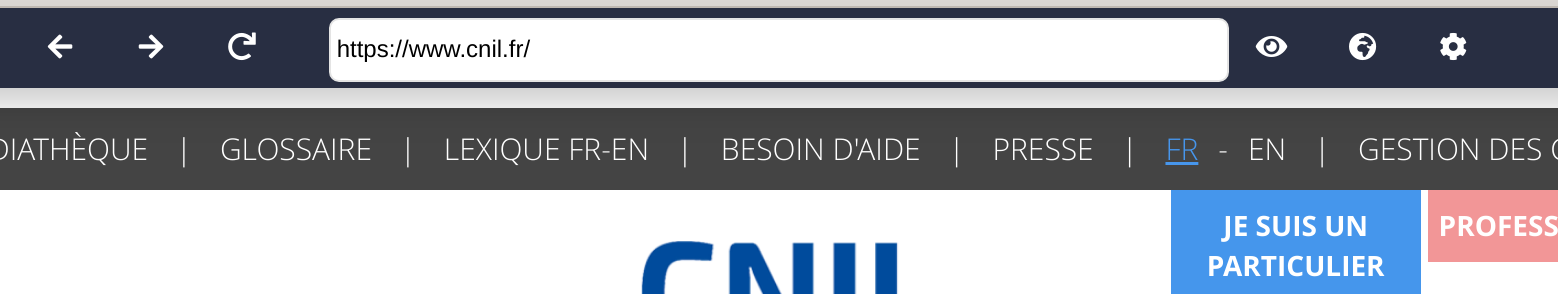
\includegraphics[width=10cm]{ressources/cookieviz.png}
\captionof{figure}{Navigateur CookieViz}
\label{navi}
\end{center}
\item Cliquer sur l'œil (figure \ref{oeil} et observer les différents traqueurs qui ont accès aux données personnelles depuis les sites visités.
\begin{center}
\centering

\includegraphics[width=2cm]{ressources/oeil.png}
\captionof{figure}{Analyse CookieViz}
\label{oeil}
\end{center}
\end{enumerate}
\end{activite}
\section{Contenu du RGPD}
\subsection{Découvrir ses connaissances}
\begin{activite}
Se rendre sur \emph{Pix} et réaliser la compétence (rose) \guill{Protéger les données personnelles et la vie privée}.
\end{activite}
\subsection{Découvrir le texte officiel}
Le \emph{RGPD} est disponible en ligne à l'adresse suivante:
\begin{center}
\url{https://www.cnil.fr/fr/reglement-europeen-protection-donnees}
\end{center}
Il semble difficile pour un particulier de lire et comprendre entièrement ce texte. C'est pourquoi la CNIL (\emph{Commission Nationale de l'Informatique et des Libertés}) propose des pages web explicatives.
\begin{center}
\url{https://www.cnil.fr/fr/rgpd-de-quoi-parle-t-on}
\end{center}
\begin{activite}
En s'aidant des liens précédents, répondre aux questions suivantes. Il est également possible d'effectuer d'autres recherches:
\begin{enumerate}
\item Combien d'articles contient le RGPD?
\item Dans quelle région du monde s'applique ce règlement?
\item Parmi les informations suivantes qu'est-ce qui peut être considéré comme une donnée personnelle?
\begin{itemize}
\item mon prénom,
\item mon numéro de téléphone,
\item l'adresse du lycée où j'étudie,
\item mon pseudo sur un forum.
\end{itemize}
\item Une entreprise américaine (Facebook) doit-elle respecter le RGPD si elle collecte les données d'un français?
\item Peut-on demander à un site web de ne plus collecter de données personnelles et de rendre celles qu'il a déjà récupérées? Quel article du RGPD détaille ce principe?
\item Quand on se rend sur un site web pour la première fois, comment est-on informé s'il collecte des données personnelles?
\item Peut-on refuser cette cette collecte?
\begin{commentprof}
droit à l'oubli article 17\\cookies
\end{commentprof}

\end{enumerate}
\end{activite}
\end{Form}
\end{document}